\documentclass[a4paper,12pt,oneside]{scrbook}
\KOMAoptions{
    chapterprefix=true,
    parskip=half,
    captions=tableheading,
    draft=false
}

% Activar números de línea
% \usepackage{lineno}
% \linenumbers
% \setlength\linenumbersep{5pt}
% \renewcommand\linenumberfont{\normalfont\tiny\sffamily\color{gray}}

\usepackage[spanish,es-nolists,es-tabla,es-noindentfirst]{babel}
\usepackage[hidelinks]{hyperref}

\renewcommand{\listtablename}{Índice de tablas}    
\renewcommand{\listfigurename}{Índice de figuras}
\newcommand*{\listofloaname}{Índice de algoritmos}

\addto\extrasspanish{
    \renewcommand{\sectionautorefname}{Apartado}
    \renewcommand{\subsectionautorefname}{Apartado}
    \renewcommand{\subsubsectionautorefname}{Apartado}
}

% Márgenes del documento
\usepackage{geometry}
\geometry{left=2cm, right=2cm, top=2cm, bottom=3.3cm}

% Interlineado 1.5
% \onehalfspacing

% Sangría 
% Ojo, la guía de KOMA-Script sugiere usar espaciado o sangría para delimitar los párrafos,
% pero no ambas cosas porque es redundante. Descomentando la siguiente línea se activa la sangría.
% \setlength{\parindent}{0.5cm}

% Configuración de fuentes
\usepackage{fontspec}
\usepackage{amsmath}
\usepackage{unicode-math}   % Incluye Latin Modern Math

\setmainfont{Latin Modern Sans}[
    Ligatures=TeX,
    % Necesario porque Latin Modern Sans no incluye estilo small caps
    SmallCapsFont=Latin Modern Roman Caps
]
\setsansfont{Latin Modern Sans}[Ligatures=TeX]
\setmonofont{Source Code Pro}[Scale=MatchLowercase]
% \setmonofont[Scale=MatchLowercase]{Fira Mono}
\newfontfamily{\lmromanfont}{Latin Modern Roman}

% Configuración de listas no numeradas
\setkomafont{itemizelabel}{\lmromanfont}
\renewcommand{\labelitemii}{$\circ$}
\renewcommand{\labelitemiii}{$\diamond$}
\renewcommand{\labelitemiv}{$\triangleright$}

% Citas
\usepackage{csquotes}
\renewcommand{\mkbegdispquote}[2]{«}
\renewcommand{\mkenddispquote}[2]{#1»#2}

%% Bibliografía
% APA (ordenada por autor, año y título)
\usepackage[style=apa,sorting=nyt,backend=biber]{biblatex}
\defbibnote{note}{Las siguientes referencias bibliográficas se presentan en orden alfabético por autor. Las referencias con más de un autor aparecen ordenadas en base al primero de los mismos.\par\bigskip}
% Numérica (ordenada por orden de aparación)
% \usepackage[style=numeric-comp,sorting=none,backend=biber]{biblatex}
% \defbibnote{note}{Las siguientes referencias bibliográficas se presentan en orden de aparición en el texto.\par\bigskip}

\addbibresource{referencias.bib}

\usepackage{caption}
\usepackage{enumitem}
\usepackage{float}
\usepackage{graphicx}
\usepackage{lipsum}
\usepackage{microtype}
\usepackage{pdflscape}
\usepackage{rotating}
\usepackage{subcaption}
\usepackage[table]{xcolor}

\usepackage{siunitx}
\newcommand{\perthousand}{‰}

% Tablas
\usepackage{array} 
\usepackage{booktabs}
\usepackage{longtable}
\usepackage{multirow}
\usepackage{tabularx}
% Definir columnas para alineación a la derecha o centro y ajuste automático
\newcolumntype{R}{>{\raggedleft\arraybackslash}X}
\newcolumntype{C}{>{\centering\arraybackslash}X}
% Definir tipos de columnas en modo matemático
% Ver pag. 3 en la documentación del paquete array:
\newcolumntype{M}{>{$}c<{$}}
\newcolumntype{L}{>{$}l<{$}}
\newcolumntype{N}{>{$}r<{$}}
% Distancia entre filas
\renewcommand*{\arraystretch}{1.5}

% Código con coloreado de sintaxis
\usepackage{scrhack}            % Para evitar un warning sobre \float@addtolist
\usepackage{listings}
\definecolor{bluekeywords}{rgb}{0.13,0.13,1}
\definecolor{greencomments}{rgb}{0,0.5,0}
\definecolor{redstrings}{rgb}{0.9,0,0}
\definecolor{punct}{rgb}{0.1,0.1,0.55}
\definecolor{delim}{rgb}{0.1,0.1,0.55}
\definecolor{numb}{rgb}{0.65,0.16,0.16}

\lstset{
  basicstyle=\ttfamily\footnotesize,  % el estilo de la fuente usado para el código
  aboveskip=12pt,                     % espacio antes del código
  belowskip=12pt,                     % espacio después del código  
  numbers=left,                       % donde poner los números de línea
  numberstyle=\tiny\color{gray},      % el estilo de los números de línea
  stepnumber=1,                       % el intervalo entre los números de línea
  numbersep=8pt,                      % cuánto espacio hay entre los números de línea y el código
  backgroundcolor=\color{white},      % el color de fondo de los cuadros de código
  showspaces=false,                   % muestra espacios agregando subrayado
  showstringspaces=false,             % subraya solo los espacios en las cadenas
  showtabs=false,                     % muestra tabulaciones agregando subrayado
  frame=leftline,                     % añade un marco alrededor del código
  framerule=0.5mm,                    % grosor de línea del marco
  rulecolor=\color{lightgray},        % si no se establece, el color del marco puede cambiar en los cuadros roto
  tabsize=2,                          % establece el tamaño de la tabulación
  captionpos=b,                       % establece la posición de la leyenda del cuadro de código
  breaklines=true,                    % líneas de ajuste automático
  breakatwhitespace=true,             % corta las líneas solo en los espacios en blanco
  keywordstyle=\color{bluekeywords}\bfseries,  % estilo para las palabras clave
  commentstyle=\color{greencomments}, % estilo para los comentarios
  stringstyle=\color{redstrings},     % estilo para las cadenas
  title=\lstname,                     % muestra el nombre de los archivos listados
  literate=
     *{0}{{{\color{numb}0}}}{1}
      {1}{{{\color{numb}1}}}{1}
      {2}{{{\color{numb}2}}}{1}
      {3}{{{\color{numb}3}}}{1}
      {4}{{{\color{numb}4}}}{1}
      {5}{{{\color{numb}5}}}{1}
      {6}{{{\color{numb}6}}}{1}
      {7}{{{\color{numb}7}}}{1}
      {8}{{{\color{numb}8}}}{1}
      {9}{{{\color{numb}9}}}{1}
      {:}{{{\color{punct}{:}}}}{1}
      {,}{{{\color{punct}{,}}}}{1}
      {\{}{{{\color{delim}{\{}}}}{1}
      {\}}{{{\color{delim}{\}}}}}{1}
      {[}{{{\color{delim}{[}}}}{1}
      {]}{{{\color{delim}{]}}}}{1},
}

%% JavaScript
% https://github.com/ghammock/LaTeX_Listings_JavaScript_ES6
\lstdefinelanguage{JavaScript}{
  morekeywords=[1]{break, continue, delete, else, for, function, if, in,
    new, return, this, typeof, var, void, while, with},
  % Literals, primitive types, and reference types.
  morekeywords=[2]{false, null, true, boolean, number, undefined,
    Array, Boolean, Date, Math, Number, String, Object},
  % Built-ins.
  morekeywords=[3]{eval, parseInt, parseFloat, escape, unescape},
  sensitive,
  morecomment=[s]{/*}{*/},
  morecomment=[l]//,
  morecomment=[s]{/**}{*/}, % JavaDoc style comments
  morestring=[b]',
  morestring=[b]"
}[keywords, comments, strings]

\lstalias[]{ES6}[ECMAScript2015]{JavaScript}

\lstdefinelanguage[ECMAScript2015]{JavaScript}[]{JavaScript}{
  morekeywords=[1]{await, async, case, catch, class, const, default, do,
    enum, export, extends, finally, from, implements, import, instanceof,
    let, static, super, switch, throw, try},
  morestring=[b]` % Interpolation strings.
}       % Estilo y definiciones para lenguajes adicionales

% Descripción de algoritmos en pseudocódigo
\usepackage[chapter]{algorithm}
\usepackage{algpseudocodex}
\floatname{algorithm}{Algoritmo}
\captionsetup[algorithm]{labelfont=bf, labelsep=default}

\newenvironment{abstract}[1][\abstractname]{
    \cleardoublepageusingstyle{empty}
    \thispagestyle{empty}
    \begin{center}\textbf{#1}\end{center}
    \begin{itshape}\par\noindent%
}
{\end{itshape}}

\newenvironment{keywords}[1][Keywords]
{\vspace{7pt}\par\noindent\textup{\textbf{#1: }}\begin{upshape}}
{\end{upshape}}

\newcommand{\license}[2]{%
\begin{center}
    \begin{minipage}{0.8\textwidth}   
        \begin{center}
            \includegraphics[width=4.66cm]{#1}\\[12pt]
            {\Large #2}
        \end{center}
    \end{minipage}
\end{center}
}

% Formato de capítulos
% Eliminar el punto y reducir el espacio entre el prefijo y el nombre del capítulo 
\renewcommand*{\chapterformat}{%
    \mbox{\chapappifchapterprefix{\nobreakspace}\thechapter
    \IfUsePrefixLine{}{\enskip}}}
\renewcommand{\chapterheadmidvskip}{\vskip 0pt}

% Formato de los títulos en figuras y tablas
\renewcommand*{\figureformat}{\figurename~\thefigure}
\renewcommand*{\tableformat}{\tablename~\thetable}

% Redefinición de las entradas de los capítulos en la tabla de contenidos
% para que aparezca el prefijo.
\let\originaladdchaptertocentry\addchaptertocentry
\renewcommand*{\addchaptertocentry}[2]{%
  \IfArgIsEmpty{#1}{% Entrada sin número
    \originaladdchaptertocentry{#1}{#2}%
  }{% Entrada con número
    % Eliminar el número y poner el prefijo directamente en el título del capítulo
    \originaladdchaptertocentry{}{\chapapp~#1\autodot\space#2}%
  }%
}

\begin{document}   

%%%%%%%%%%%%%%%%%%%%%%%%%%%%%%%%%%%%%%%%%%%%%%%%%%%%%%%%%%%%%%%%%%%%%%%%%%%%%%%
% Portada y metadatos
%%%%%%%%%%%%%%%%%%%%%%%%%%%%%%%%%%%%%%%%%%%%%%%%%%%%%%%%%%%%%%%%%%%%%%%%%%%%%%%

% Metadatos del PDF
\hypersetup{
    pdftitle='Título del trabajo',
    pdfauthor='Nombre y Apellidos',
    pdfsubject={Trabajo de Fin de Grado},
}

\pagestyle{empty}
\newcommand{\HRule}{\rule{\linewidth}{0.3mm}}
{
    \setlength{\parindent}{0mm}
    \setlength{\parskip}{0mm}
    
    \vspace*{1.20cm}
    
\includegraphics[width=9.81cm]{images/logos/escuela-ingenieria-tecnologia-original}
    \vspace*{\stretch{0.9}}
    
    {\centering
    \fontsize{32pt}{32pt}\selectfont Trabajo de Fin de Grado\\[10pt]
    \fontsize{20pt}{20pt}\selectfont Grado en Ingeniería Informática\par}
    \HRule\vspace*{-2mm}
    \begin{flushright}
        {\fontsize{32pt}{32pt}\selectfont Título del trabajo\par
        \vspace*{3mm}
        \fontsize{18pt}{18pt}\selectfont \textit{Title in English}\par
        \vspace*{11mm}
        \fontsize{16pt}{16pt}\selectfont Nombre y Apellidos
        }\vspace*{12mm}
    \end{flushright}
    \HRule
    
    \vspace*{\stretch{1}}
    \begin{center}
        \fontsize{18pt}{18pt}\selectfont La Laguna, \today
    \end{center}
}

%%%%%%%%%%%%%%%%%%%%%%%%%%%%%%%%%%%%%%%%%%%%%%%%%%%%%%%%%%
% Certificado
%%%%%%%%%%%%%%%%%%%%%%%%%%%%%%%%%%%%%%%%%%%%%%%%%%%%%%%%%%
\frontmatter
\cleardoublepageusingstyle{empty}
\thispagestyle{empty}

{
\setlength\parindent{0pt}
    D. \textbf{Nombre Apellido1 Apellido2}, profesor Titular de Universidad adscrito al Departamento de Nombre del Departamento de la Universidad de La Laguna, como tutor
    
    \bigskip
    D. \textbf{Nombre Apellido1 Apellido2}, profesor Titular de Universidad adscrito al Departamento de Nombre del Departamento de la Universidad de La Laguna, como cotutor.
    
    \bigskip
    \bigskip
    \textbf{C E R T I F I C A (N)}

    \bigskip
    Que la presente memoria titulada:
    
    \bigskip
    \begin{quote}
    \textit{``Título del Trabajo''}
    \end{quote}
    
    \bigskip
    \noindent ha sido realizada bajo su dirección por D. \textbf{Nombre Apellido1 Apellido2}.
    
    \bigskip
    Y para que así conste, en cumplimiento de la legislación vigente y a los efectos
    oportunos, firman la presente en La Laguna a \today
}

%%%%%%%%%%%%%%%%%%%%%%%%%%%%%%%%%%%%%%%%%%%%%%%%%%%%%%%%%%
% Agradecimientos
%%%%%%%%%%%%%%%%%%%%%%%%%%%%%%%%%%%%%%%%%%%%%%%%%%%%%%%%%%
\cleardoublepageusingstyle{empty}
\thispagestyle{empty}

\begin{flushright}
    \setlength{\parindent}{0mm}

    {\LARGE Agradecimientos}
    \vspace{15mm}
    
    \begin{large}
        \begin{minipage}{0.3\textwidth}
            \begin{flushright}
            XXX
            
            XXX
            
            XXX
            
            XXX
            \end{flushright}
        \end{minipage}
    \end{large}
\end{flushright}

%%%%%%%%%%%%%%%%%%%%%%%%%%%%%%%%%%%%%%%%%%%%%%%%%%%%%%%%%%
% Licencia
%%%%%%%%%%%%%%%%%%%%%%%%%%%%%%%%%%%%%%%%%%%%%%%%%%%%%%%%%%
\cleardoublepageusingstyle{empty}
\thispagestyle{empty}

{\noindent\LARGE Licencia}
\vspace{15mm}

\textcolor{red}{Elige una licencia y elimina el testo de opciones.}
\bigskip

\textcolor{red}{• Si NO quiere permitir que se compartan las adaptaciones de tu obra y NO quieres permitir usos comerciales de tu obra, indica:}

\license{images/licenses/by-nc-nd.eu}{© Esta obra está bajo una licencia de Creative Commons Reconocimiento-NoComercial-SinObraDerivada 4.0 Internacional.}

\bigskip
\textcolor{red}{• Si quiere permitir que se compartan las adaptaciones de tu obra mientras se comparta de la misma manera y NO quieres permitir usos comerciales de tu obra, indica:}

\license{images/licenses/by-nc-sa.eu}{© Esta obra está bajo una licencia de Creative Commons Reconocimiento-NoComercial-CompartirIgual 4.0 Internacional.}
        
\bigskip
\textcolor{red}{• Si quiere permitir que se compartan las adaptaciones de tu obra y NO quieres permitir usos comerciales de tu obra, indica:}

\license{images/licenses/by-nc.eu}{© Esta obra está bajo una licencia de Creative Commons Reconocimiento-NoComercial 4.0 Internacional.}
    
\bigskip
\textcolor{red}{• Si NO quiere permitir que se compartan las adaptaciones de tu obra y quieres permitir usos comerciales de tu obra, indica:}

\license{images/licenses/by-nd}{© Esta obra está bajo una licencia de Creative Commons Reconocimiento-SinObraDerivada 4.0 Internacional.}

\bigskip
\textcolor{red}{• Si quiere permitir que se compartan las adaptaciones de tu obra mientras se comparta de la misma manera y quieres permitir usos comerciales de tu obra (licencia de Cultura Libre) indica:}

\license{images/licenses/by-sa}{© Esta obra está bajo una licencia de Creative Commons Reconocimiento-CompartirIgual 4.0 Internacional.}  

\bigskip
\textcolor{red}{• Si quiere permitir que se compartan las adaptaciones de tu obra y quieres permitir usos comerciales de tu obra (licencia de Cultura Libre) indica:}

\license{images/licenses/by}{© Esta obra está bajo una licencia de Creative Commons Reconocimiento 4.0 Internacional.}

%%%%%%%%%%%%%%%%%%%%%%%%%%%%%%%%%%%%%%%%%%%%%%%%%%%%%%%%%%
% Resumen
%%%%%%%%%%%%%%%%%%%%%%%%%%%%%%%%%%%%%%%%%%%%%%%%%%%%%%%%%%
\begin{abstract}
El objetivo de este trabajo ha sido... bla, bla, bla, bla, bla, bla, bla, bla, bla...

La competencia [E6], que figura en la guía docente, indica que en la memoria del trabajo se ha de incluir: antecedentes, problemática o estado del arte, objetivos, fases y desarrollo del proyecto, conclusiones, y líneas futuras.

Se ha incluido el apartado de 'Licencia' con todas las posibles licencias abiertas (Creative Commons). En el caso en que se decida hacer público el contenido de la memoria, habrá que elegir una de ellas (y borrar las demás). La decisión de hacer pública o no la memoria se indica en el momento de subir la memoria a la Sede Electrónica de la ULL, paso necesario en el proceso de presentación del TFG.

El documento de memoria debe tener un máximo de 50 páginas.

No se deben dejar páginas en blanco al comenzar un capítulo, ya que el documento no está pensado para ser impreso sino visionado con un lector de PDF.

También es recomendable usar márgenes pequeños, ya que, al firmar digitalmente por la Sede Electrónica, se coloca un marco alrededor del texto original.

El tipo de letra base ha de ser de 12 pt.

\begin{keywords}[Palabras clave]
Palabra reservada1, Palabra reservada2,...
\end{keywords}
\end{abstract}

%%%%%%%%%%%%%%%%%%%%%%%%%%%%%%%%%%%%%%%%%%%%%%%%%%%%%%%%%
\cleardoublepageusingstyle{empty}
\thispagestyle{empty}

\begin{abstract}[Abstract]
Here should be the abstract in a foreing language...

\begin {keywords}
Keyword1, Keyword2, Keyword3,...
\end{keywords}
\end{abstract}

%%%%%%%%%%%%%%%%%%%%%%%%%%%%%%%%%%%%%%%%%%%%%%%%%%%%%%%%%
\pagestyle{plain}
\cleardoublepage
\setcounter{page}{1} 

\tableofcontents
\listoffigures
\listoftables
%\listofalgorithms

%%%%%%%%%%%%%%%%%%%%%%%%%%%%%%%%%%%%%%%%%%%%%%%%%%%%%%%%%%
% Contenidos
%%%%%%%%%%%%%%%%%%%%%%%%%%%%%%%%%%%%%%%%%%%%%%%%%%%%%%%%%%
\mainmatter

\input{01-introducción}
\chapter{Título del Capítulo 2}
\label{ch:capítulo-dos}

Los capítulos intermedios sirven para cubrir los siguientes aspectos: antecedentes, problemática o estado del arte, objetivos, fases y desarrollo del proyecto.

En el capítulo anterior se ha introducido la \autoref{fig:introducción} y en este la \autoref{fig:otra}. 

\section{Primera sección de otro capítulo}
\label{sec:primera_sección}

\begin{figure}[htbp]
   \centering
   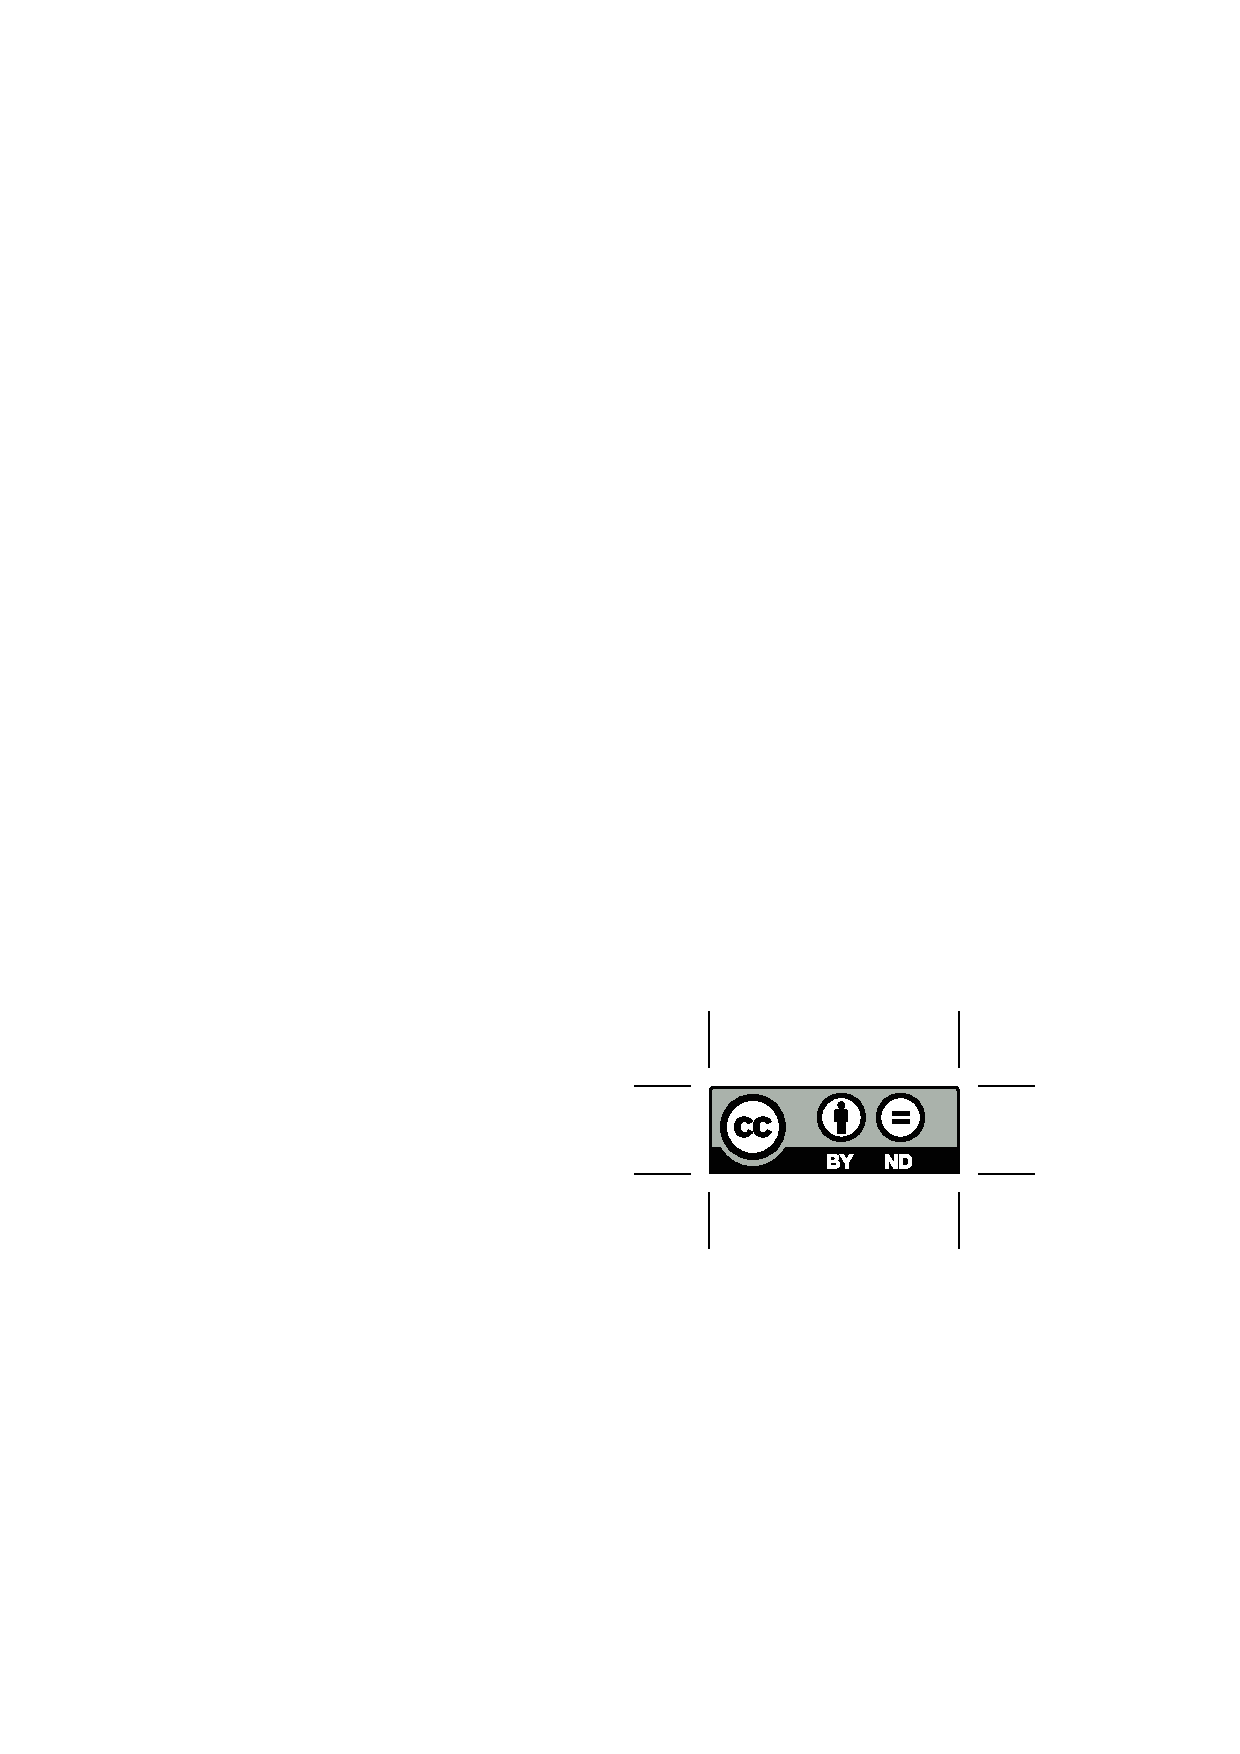
\includegraphics[width=0.5\linewidth]{images/licenses/by-nd}
   \caption{Otra figura.}
   \label{fig:otra}
\end{figure}

\lipsum[3]

\subsection{Primera subsección}

\lipsum[4]

\subsection{Segunda subsección}

\lipsum[5]

\section{Segunda sección de otro capítulo}

\lipsum[6-7]



\chapter{Título del Capítulo 3}
\label{ch:capítulo-tres}

Los capítulos intermedios sirven para cubrir los siguientes aspectos: antecedentes, problemática o estado del arte, objetivos, fases y desarrollo del proyecto.

\section{Primera sección de este capítulo}

\lipsum[-2]

\section{Segundo apartado de este capítulo}

\lipsum[3]

\section{Tercer apartado de este capítulo}

\lipsum[4]
\chapter{Título del Capítulo 4}
\label{ch:capítulo-cuatro}

Los capítulos intermedios sirven para cubrir los siguientes aspectos: antecedentes, problemática o estado del arte, objetivos, fases y desarrollo del proyecto.

En el \autoref{ch:introducción} se comentó lo que \cite{examplearticle} dijo al respecto. Aquí vamos a profundizar en una de sus afirmaciones más controvertidas:

\begin{displayquote}[Albert Einstein]
\lipsum[7]
\end{displayquote}

Es decir que \textquote{erat ac sagittis sempe}, lo que se ilustra en el esquema de la \autoref{fig:otra}.

\lipsum[2]
\chapter{Conclusiones y líneas futuras}
\label{ch:conclusiones}

Este capítulo es obligatorio. Toda memoria de trabajo de fin de grado debe incluir unas conclusiones y unas líneas de trabajo futuro.
\chapter{Summary and Conclusions}
\label{ch:conclusions}

This chapter is compulsory. The memory should include an extended summary and conclusions in English.
\chapter{Presupuesto}
\label{ch:presupuesto}

Este capítulo es obligatorio. Toda memoria de trabajo de fin de grado debe incluir un presupuesto.

\section{Sección Uno}

\begin{table}[!ht]
\centering
\caption{Presupuesto de Equipos y Licencias}
\begin{tabularx}{0.8\textwidth}{Xcr}
    \toprule
    \textbf{Descripción} & \textbf{Cantidad} & \textbf{Coste (€)} \\
    \midrule
    Portátil & 1 & 900,00 \\
    Licencia de Software de Desarrollo (IDE) & 1 & 100,00 \\
    Licencia de Software de Diseño Gráfico & 1 & 50,00 \\
    Compra de Componentes Adicionales & 1 & 150,00 \\
    Servicios en la Nube & 12 meses & 240 \\
    \midrule
    \textbf{Subtotal de Equipos y Licencias} & & \textbf{1440,00} \\
    \bottomrule
\end{tabularx}
\end{table}

\begin{table}[!ht]
\centering
\caption{Coste de Mano de Obra}
\begin{tabularx}{0.8\textwidth}{Xcr}
    \toprule
    \textbf{Descripción} & \textbf{Horas} & \textbf{Coste (€)} \\
    \midrule
    Precio por Hora & & 20,00 \\
    Total de Horas de Trabajo & 100 & \\
    \midrule
    \textbf{Costo Total del Trabajo Humano} & & \textbf{2000,00} \\
    \bottomrule
\end{tabularx}
\end{table}

\begin{table}[!ht]
\centering
\caption{Coste Total del Proyecto}
\label{tbl:presupuesto}
\begin{tabularx}{0,8\textwidth}{Xr}
    \toprule
    \textbf{Descripción} & \textbf{Coste Total (€)} \\
    \midrule
    Subtotal de Equipos y Licencias & 1440,00 \\
    Costo Total del Trabajo & 2000,00 \\
    \midrule
    \textbf{Coste Total del Proyecto} & \textbf{3440,00} \\
    \bottomrule
\end{tabularx}
\end{table}


\appendix

\chapter{Título del Apéndice 1}
\label{ch:apéndice-uno}

\section{Algoritmo XXX}
\label{sec:algoritmo-xxx}

Ejemplo de código con coloreado de sintaxis:

\begin{lstlisting}[language=C++]
#include <iostream>

int main()
{
  // Imprime "Hello, world!" en la consola
  std::cout << "Hello, world!\n";
  return 0;
}
\end{lstlisting}

\section{Archivo XXY}
\label{sec:archivo-xxy}

Ejemplo de JSON usando el mismo entorno de coloreado de sintaxis:

\begin{lstlisting}
{
    "nombre": "John Doe",
    "edad": 30,
    "ciudad": "Nueva York",
    "hobbies": [
        "lectura",
        "jardinería",
        "ciclismo"
    ],
    "empleo": {
        "título": "Ingeniero de Software",
        "empresa": "TechCorp"
    }
}
\end{lstlisting}
 
\section{Algoritmo YYY}
\label{sec:algoritmo-yyy}

Este es el clásico entorno \texttt{verbatim}, sin coloreado pero con fuente monoespaciada:

\begin{center}
\begin{footnotesize}
\begin{verbatim}

/***********************************************************************************
 *
 * Fichero .h
 *
 ***********************************************************************************
 *
 * AUTORES
 *
 * FECHA
 *
 * DESCRIPCION
 *
 *
 ************************************************************************************/
 
\end{verbatim}
\end{footnotesize}
\end{center}

\section{Algoritmo ZZZ}
\label{sec:algoritmo-zzz}

Ejemplo de entorno para describir algoritmos en pseudocódigo:

\begin{algorithm}[htpb]
    \caption{Cálculo del factorial de un número}\label{alg:factorial}
    \begin{algorithmic}[1]
        \State \textbf{Entrada:} Un entero $n$
        \State \textbf{Salida:} El factorial de $n$
        \Function{Factorial}{$n$}\Comment{El factorial de n}
            \If{$n \leq 1$}
                \State \Return $1$\Comment{El factorial de 0 o 1 es 1}
            \Else
                \State \Return $n \times$ \Call{Factorial}{n-1}
            \EndIf
        \EndFunction
    \end{algorithmic}
\end{algorithm}

Otra forma de describir algoritmos es utilizar entornos \texttt{lstlisting} y emplear una sintaxis de pseudocódigo similar a alguno de los lenguajes soportados por este paquete, como Python o Pascal.
\chapter{Título del Apéndice 2}
\label{ch:apéndice-dos}

\section{Otro apéndice: Sección 1}
\lipsum[2]

\section{Otro apéndice: Sección 2}
\lipsum[3]

%%%%%%%%%%%%%%%%%%%%%%%%%%%%%%%%%%%%%%%%%%%%%%%%%%%%%%%%%%
% Bibliografía
%%%%%%%%%%%%%%%%%%%%%%%%%%%%%%%%%%%%%%%%%%%%%%%%%%%%%%%%%%
\backmatter

\printbibliography[prenote=note]
%%%%%%%%%%%%%%%%%%%%%%%%%%%%%%%%%%%%%%%%%%%%%%%%%%%%%%%%%%

\end{document}

